\documentclass[DIN, pagenumber=false, fontsize=11pt, parskip=half]{scrartcl}
\usepackage[UTF8]{ctex}  % 中文支持
% \usepackage{ngerman}
\usepackage[utf8]{inputenc}
\usepackage[T1]{fontenc}
\usepackage{textcomp}
\usepackage{graphicx}

\usepackage{xcolor} % Required for custom red

\usepackage{geometry} % Custom margins

\usepackage{tocloft} % Modifying the table of contents

% for matlab code
% bw = blackwhite - optimized for print, otherwise source is colored
\usepackage[framed,numbered,bw]{mcode}
\usepackage[most]{tcolorbox}
% for other code
%\usepackage{listings}

\setlength{\parindent}{0em}

% set section in CM
\setkomafont{section}{\normalfont\bfseries\Large}

\newcommand{\mytitle}[1]{{\noindent\Large\textbf{#1}}}
\newcommand{\mysection}[1]{\textbf{\section*{#1}}}
\newcommand{\mysubsection}[2]{\romannumeral #1) #2}

\newtcolorbox{parchmentquote}{
    enhanced,
    colback=orange!5!white,   % 浅米黄色背景
    colframe=orange!50!black,
    boxrule=0.5pt,
    arc=2pt,                  % 细微圆角
    boxsep=5pt,
    before skip=10pt,
    after skip=10pt,
    fontupper=\itshape,
    borderline west={2pt}{0pt}{orange!80!black} % 加厚的左装饰线
}
%===================================
\begin{document}

\noindent\textbf{课后总结} \hfill \textbf{face-to-face course}\\
primary school \hfill Liu\\

\mytitle{近日总结 \hfill \today}
\newline
\begin{parchmentquote}
	能够使用草稿纸进行笔算，这个习惯已经很好。
    读题这个需要慢慢提升。

\end{parchmentquote}


%===================================
\section{一些细节}

\subsection{竖式书写规范} 
尽量在竖式与算式之间有点空，这样商会更加清晰、不至于太紧凑
\begin{figure}[htbp]
    \centering
    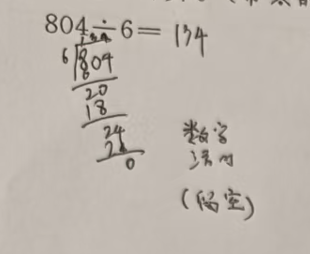
\includegraphics[width=0.8\textwidth]{image_123.png}
    \caption{截图}
    \label{fig:example}
\end{figure}


\subsection{数字与汉字的区分} 
一般是\textbf{一位数、两位数、三位数}，
考试时候尽量写汉字，虽然生活中2位数不错，这是考试细节

\section{题型总结}

\subsection{长度不变或者周长不变}
把一条铁丝折成一个三角形、长方形、正方形，这个铁丝的长度不变，就是周长不变，找好等量关系
\subsection{商的简单判定}
${80? \div 5}$ 能简单判定一定三位数，因为百位数字是8大于5，所以商一定三位数
\end{document}